\documentclass[12pt,letterpaper]{article}\usepackage[]{graphicx}\usepackage[]{color}
%% maxwidth is the original width if it is less than linewidth
%% otherwise use linewidth (to make sure the graphics do not exceed the margin)
\makeatletter
\def\maxwidth{ %
  \ifdim\Gin@nat@width>\linewidth
    \linewidth
  \else
    \Gin@nat@width
  \fi
}
\makeatother

\definecolor{fgcolor}{rgb}{0.345, 0.345, 0.345}
\newcommand{\hlnum}[1]{\textcolor[rgb]{0.686,0.059,0.569}{#1}}%
\newcommand{\hlstr}[1]{\textcolor[rgb]{0.192,0.494,0.8}{#1}}%
\newcommand{\hlcom}[1]{\textcolor[rgb]{0.678,0.584,0.686}{\textit{#1}}}%
\newcommand{\hlopt}[1]{\textcolor[rgb]{0,0,0}{#1}}%
\newcommand{\hlstd}[1]{\textcolor[rgb]{0.345,0.345,0.345}{#1}}%
\newcommand{\hlkwa}[1]{\textcolor[rgb]{0.161,0.373,0.58}{\textbf{#1}}}%
\newcommand{\hlkwb}[1]{\textcolor[rgb]{0.69,0.353,0.396}{#1}}%
\newcommand{\hlkwc}[1]{\textcolor[rgb]{0.333,0.667,0.333}{#1}}%
\newcommand{\hlkwd}[1]{\textcolor[rgb]{0.737,0.353,0.396}{\textbf{#1}}}%

\usepackage{framed}
\makeatletter
\newenvironment{kframe}{%
 \def\at@end@of@kframe{}%
 \ifinner\ifhmode%
  \def\at@end@of@kframe{\end{minipage}}%
  \begin{minipage}{\columnwidth}%
 \fi\fi%
 \def\FrameCommand##1{\hskip\@totalleftmargin \hskip-\fboxsep
 \colorbox{shadecolor}{##1}\hskip-\fboxsep
     % There is no \\@totalrightmargin, so:
     \hskip-\linewidth \hskip-\@totalleftmargin \hskip\columnwidth}%
 \MakeFramed {\advance\hsize-\width
   \@totalleftmargin\z@ \linewidth\hsize
   \@setminipage}}%
 {\par\unskip\endMakeFramed%
 \at@end@of@kframe}
\makeatother

\definecolor{shadecolor}{rgb}{.97, .97, .97}
\definecolor{messagecolor}{rgb}{0, 0, 0}
\definecolor{warningcolor}{rgb}{1, 0, 1}
\definecolor{errorcolor}{rgb}{1, 0, 0}
\newenvironment{knitrout}{}{} % an empty environment to be redefined in TeX

\usepackage{alltt}
\usepackage[utf8]{inputenc}
\usepackage[margin=.7in]{geometry}
\usepackage{graphicx}
\usepackage{titling}
\usepackage{amsmath}
\usepackage{amsfonts}
\usepackage{amssymb}
\renewcommand{\theenumiv}{\arabic{enumiv}}
\setlength{\droptitle}{-5em}
\author{Maurice Diesendruck\vspace{-2ex}}
\title{StatMod2 - Hierarchical Models and Shrinkage - Exercises 4\vspace{-1ex}}
\IfFileExists{upquote.sty}{\usepackage{upquote}}{}
\begin{document}
\maketitle
\setcounter{section}{1}

\section{Price Elasticity of Demand}

\subsection{Model}
Here, I used a linear model in the log-log form, and computed Gibbs sampling
using JAGS. Exact likelihood and priors are shown below:\\

\begin{knitrout}
\definecolor{shadecolor}{rgb}{0.969, 0.969, 0.969}\color{fgcolor}\begin{kframe}
\begin{alltt}
\hlcom{# CONTENTS OF MODEL FILE}
model \{
\hlkwd{for} (j in 1:N) \{
  LOG.Q[j] ~ \hlkwd{dnorm}(mean[j], sigsq)
  mean[j] <- beta[1] + beta[2]*log.P[j] + beta[3]*disp[j] +
             beta[4]*cross[j]
\}
beta[1] ~ \hlkwd{dnorm}(0,0.001) \hlcom{# Diffuse priors}
beta[2] ~ \hlkwd{dnorm}(0,0.001)
beta[3] ~ \hlkwd{dnorm}(0,0.001)
beta[4] ~ \hlkwd{dnorm}(0,0.001)
sigsq ~ \hlkwd{dgamma}(1, 1)
\}
\end{alltt}
\end{kframe}
\end{knitrout}

\subsection{Gibbs Sampler}

The following Gibbs sampler (using JAGS), produces chains for variables
$log\alpha_i$, $\beta_i$, $\gamma_i$, and $\delta_i$. In the code, these
four variables are called $log.a$, $b$, $g$, and $d$.

\begin{knitrout}
\definecolor{shadecolor}{rgb}{0.969, 0.969, 0.969}\color{fgcolor}\begin{kframe}
\begin{alltt}
\hlcom{# StatMod2 - Cheese - JAGS Version}

\hlkwd{library}\hlstd{(rjags)}
\hlkwd{library}\hlstd{(boot)}
\hlkwd{library}\hlstd{(VGAM)}
\hlkwd{library}\hlstd{(MASS)}

\hlcom{# Fetch and prepare data.}
\hlstd{path} \hlkwb{<-} \hlkwd{paste}\hlstd{(}\hlstr{"~/Google Drive/2. SPRING 2015/STAT MOD 2 - Prof Scott/"}\hlstd{,}
              \hlstr{"hierarch-shrinkage/cheese"}\hlstd{,} \hlkwc{sep}\hlstd{=}\hlstr{""}\hlstd{)}
\hlkwd{setwd}\hlstd{(path)}
\hlstd{data} \hlkwb{<-} \hlkwd{read.csv}\hlstd{(}\hlstr{"cheese.csv"}\hlstd{)}
\hlstd{data}\hlopt{$}\hlstd{log.Q} \hlkwb{<-} \hlkwd{log}\hlstd{(data}\hlopt{$}\hlstd{vol)}
\hlstd{data}\hlopt{$}\hlstd{log.P} \hlkwb{<-} \hlkwd{log}\hlstd{(data}\hlopt{$}\hlstd{price)}
\hlkwd{attach}\hlstd{(data)}
\hlstd{n} \hlkwb{<-} \hlkwd{dim}\hlstd{(data)[}\hlnum{1}\hlstd{]}
\hlstd{store.names} \hlkwb{<-} \hlkwd{unique}\hlstd{(data}\hlopt{$}\hlstd{store)}

\hlcom{# Execute Gibbs sampler for all stores.}
\hlstd{Execute} \hlkwb{<-} \hlkwa{function}\hlstd{() \{}
  \hlstd{num.stores} \hlkwb{<-} \hlkwd{length}\hlstd{(store.names)}
  \hlcom{# Make container for store name, and means of 4 vars: log.a, b, g, d.}
  \hlstd{PARAMS.BY.STORE} \hlkwb{<-} \hlkwd{matrix}\hlstd{(}\hlnum{NA}\hlstd{,} \hlkwc{nrow}\hlstd{=num.stores,} \hlkwc{ncol}\hlstd{=}\hlnum{5}\hlstd{)}
  \hlkwa{for} \hlstd{(i} \hlkwa{in} \hlnum{1}\hlopt{:}\hlstd{num.stores) \{}
    \hlstd{name} \hlkwb{<-} \hlkwd{toString}\hlstd{(store.names[i])}
    \hlstd{store.data} \hlkwb{<-} \hlstd{data[}\hlkwd{which}\hlstd{(data}\hlopt{$}\hlstd{store}\hlopt{==}\hlstd{name),]}
    \hlstd{PARAMS.BY.STORE[i,]} \hlkwb{<-} \hlkwd{c}\hlstd{(name,} \hlkwd{Gibbs}\hlstd{(store.data, name))}
  \hlstd{\}}
  \hlkwd{return} \hlstd{(PARAMS.BY.STORE)}
\hlstd{\}}

\hlstd{Gibbs} \hlkwb{<-} \hlkwa{function}\hlstd{(}\hlkwc{store.data}\hlstd{,} \hlkwc{name}\hlstd{) \{}
  \hlcom{# Set up JAGS model over 3 variables.}
  \hlstd{jagsmodel} \hlkwb{<-} \hlkwd{jags.model}\hlstd{(}\hlkwc{file}\hlstd{=}\hlstr{"cheese-jags-model.txt"}\hlstd{,}
                           \hlkwc{data}\hlstd{=}\hlkwd{list}\hlstd{(}\hlkwc{LOG.Q}\hlstd{=store.data}\hlopt{$}\hlstd{log.Q,}
                                \hlkwc{log.P}\hlstd{=store.data}\hlopt{$}\hlstd{log.P,}
                                \hlkwc{disp}\hlstd{=store.data}\hlopt{$}\hlstd{disp,}
                                \hlkwc{cross}\hlstd{=store.data}\hlopt{$}\hlstd{log.P}\hlopt{*}\hlstd{store.data}\hlopt{$}\hlstd{disp,}
                                \hlkwc{N}\hlstd{=}\hlkwd{length}\hlstd{(store.data}\hlopt{$}\hlstd{log.Q)),}
                           \hlkwc{n.chains}\hlstd{=}\hlnum{2}\hlstd{)}

  \hlcom{# Fit jagsmodel.}
  \hlstd{jagsfit} \hlkwb{<-} \hlkwd{jags.samples}\hlstd{(jagsmodel,}
                          \hlkwc{variable.names}\hlstd{=}\hlkwd{c}\hlstd{(}\hlstr{"beta"}\hlstd{),}
                          \hlkwc{n.iter}\hlstd{=}\hlnum{100000}\hlstd{,} \hlkwc{thin}\hlstd{=}\hlnum{1000}\hlstd{)}

  \hlcom{# Create traceplots for beta chains.}
  \hlkwd{par}\hlstd{(}\hlkwc{mfrow}\hlstd{=}\hlkwd{c}\hlstd{(}\hlnum{4}\hlstd{,} \hlnum{2}\hlstd{))}
  \hlstd{ref} \hlkwb{<-} \hlkwd{c}\hlstd{(}\hlstr{"log.a"}\hlstd{,} \hlstr{"b"}\hlstd{,} \hlstr{"g"}\hlstd{,} \hlstr{"d"}\hlstd{)}
  \hlkwa{for} \hlstd{(i} \hlkwa{in} \hlnum{1}\hlopt{:}\hlnum{4}\hlstd{) \{}
    \hlcom{# jagsfit$var takes three arguments: parameter, row, chain.}
    \hlkwd{plot}\hlstd{(jagsfit}\hlopt{$}\hlstd{beta[i,,}\hlnum{1}\hlstd{],} \hlkwc{type}\hlstd{=}\hlstr{"l"}\hlstd{,} \hlkwc{col}\hlstd{=}\hlstr{"red"}\hlstd{,} \hlkwc{ylab}\hlstd{=}\hlstr{""}\hlstd{,}
         \hlkwc{main}\hlstd{=}\hlkwd{bquote}\hlstd{(}\hlkwd{.}\hlstd{(name)} \hlopt{~} \hlkwd{.}\hlstd{(ref[i])} \hlopt{==} \hlkwd{.}\hlstd{(i)))}
    \hlkwd{lines}\hlstd{(jagsfit}\hlopt{$}\hlstd{beta[i,,}\hlnum{2}\hlstd{],} \hlkwc{type}\hlstd{=}\hlstr{"l"}\hlstd{,} \hlkwc{col}\hlstd{=}\hlstr{"blue"}\hlstd{)}
    \hlkwd{plot}\hlstd{(}\hlkwd{density}\hlstd{(jagsfit}\hlopt{$}\hlstd{beta[i,,]),} \hlkwc{type}\hlstd{=}\hlstr{"l"}\hlstd{,}
         \hlkwc{main}\hlstd{=}\hlkwd{bquote}\hlstd{(}\hlkwd{.}\hlstd{(name)} \hlopt{~} \hlkwd{.}\hlstd{(ref[i])} \hlopt{==} \hlkwd{.}\hlstd{(i)))}
  \hlstd{\}}

  \hlstd{mean.params} \hlkwb{<-} \hlkwd{rowMeans}\hlstd{(jagsfit}\hlopt{$}\hlstd{beta[,,}\hlnum{1}\hlstd{])}
  \hlkwd{return} \hlstd{(mean.params)}
\hlstd{\}}

\hlstd{PARAMS.BY.STORE} \hlkwb{<-} \hlkwd{Execute}\hlstd{()}
\end{alltt}
\end{kframe}
\end{knitrout}

Here is an example of the output for one store:\\

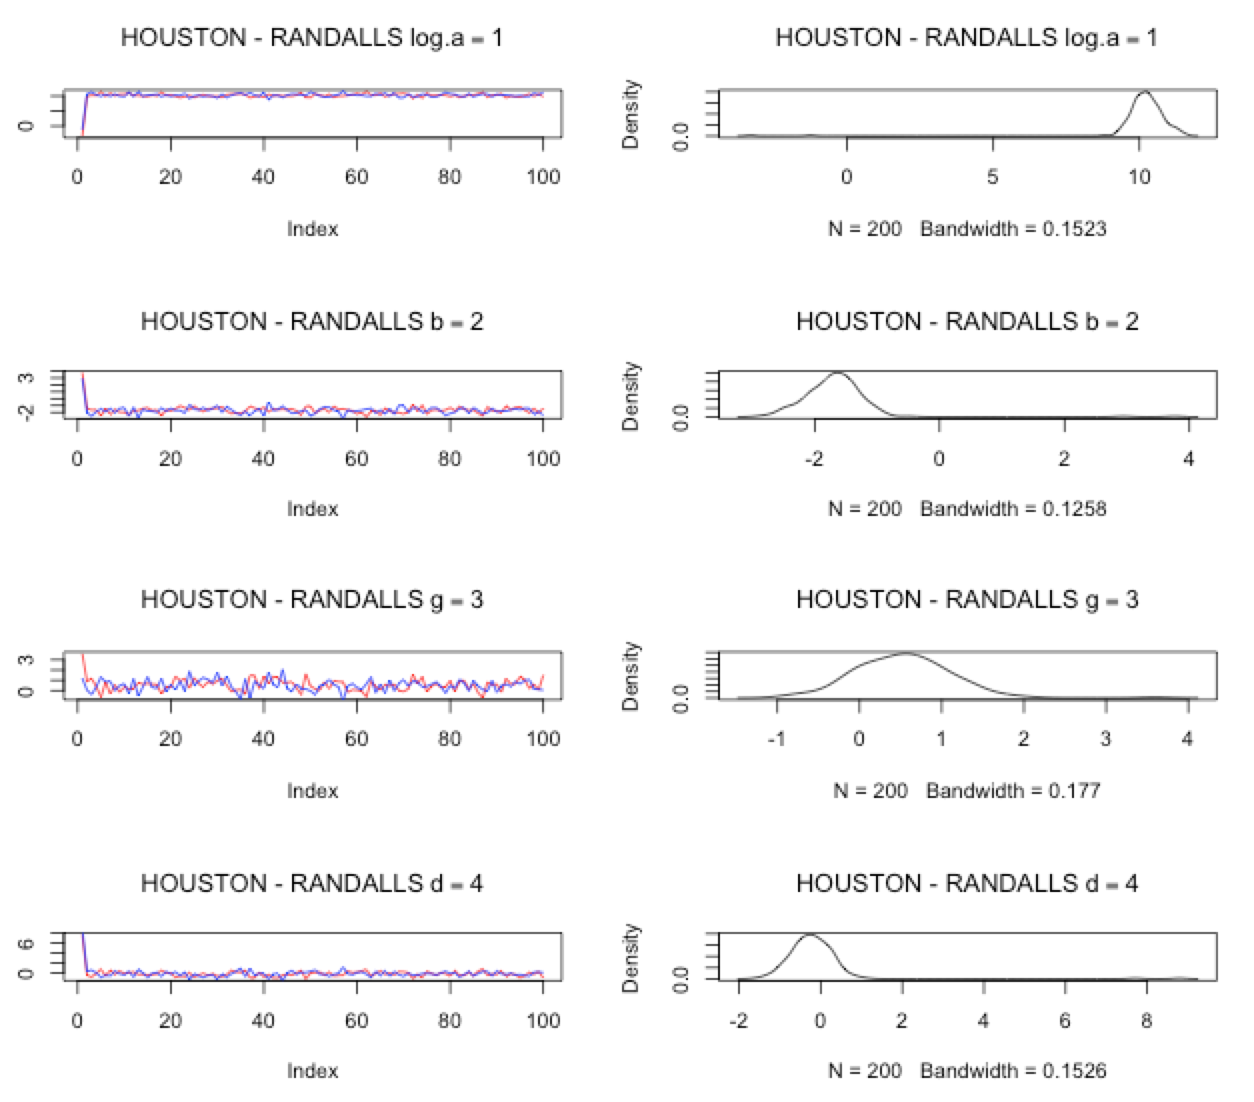
\includegraphics[width=\textwidth]{store-example.png}

The variable $PARAMS.BY.STORE$, holds the chain means for each variable. A
subset of this matrix is shown below:\\

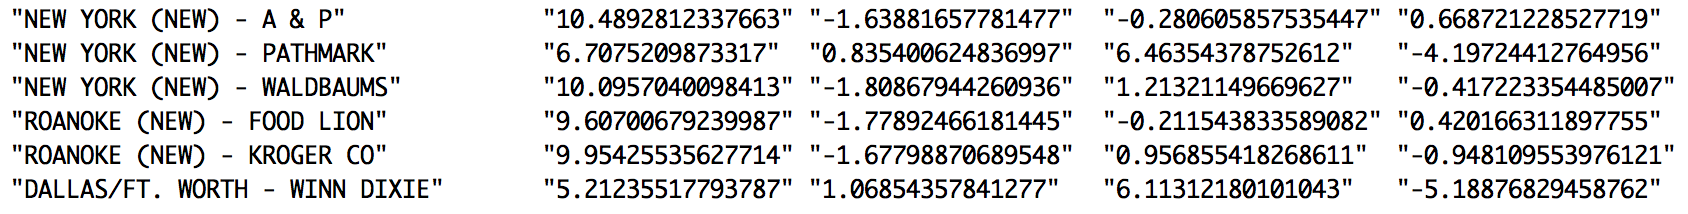
\includegraphics[width=\textwidth]{PARAMS-BY-STORE-example.png}

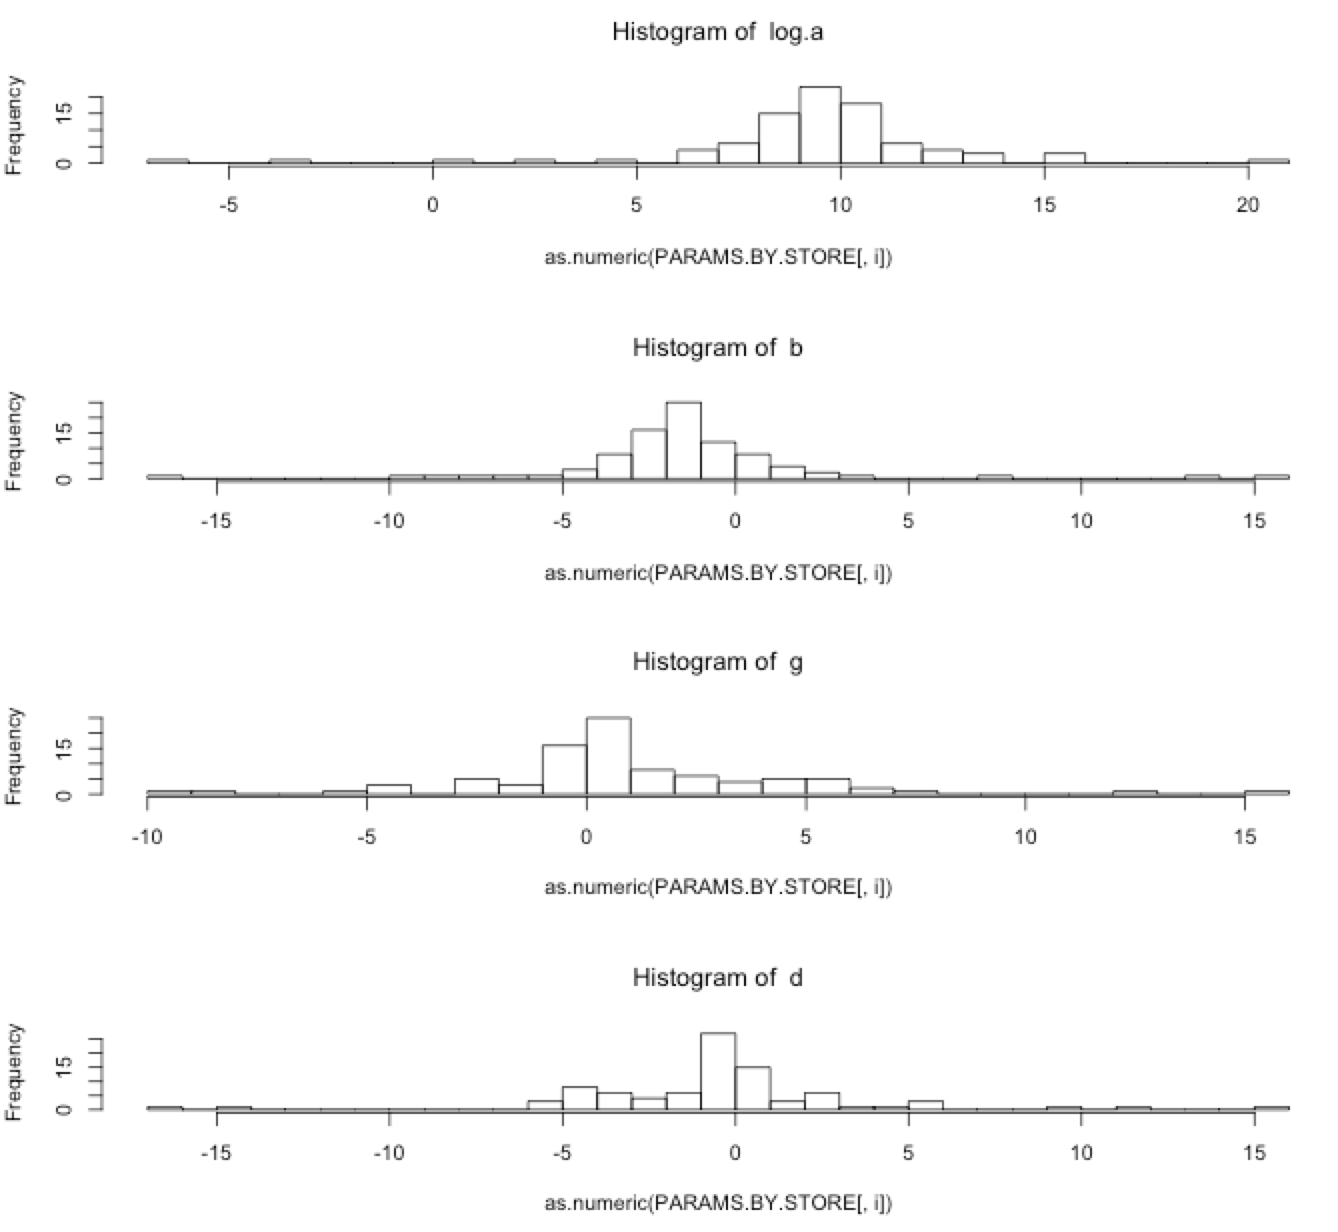
\includegraphics[width=\textwidth]{inspect-results.png}

\end{document}


